\setcounter{secnumdepth}{1}

\begin{table*}[!t]
\centering
\scriptsize
\setlength{\tabcolsep}{3pt}
\begin{tabular}{@{}p{0.36\linewidth}p{\dimexpr0.64\linewidth-2\tabcolsep\relax}@{}}
\toprule
Features (41 scalar inputs in total) & Operationalisation\\
\midrule
\textbf{Text and language (7):}
Comment length; positive and negative sentiment; maximum toxicity; length-adjusted lexical diversity; length-adjusted reading difficulty; URL present &
$\log(1+$ word count$)$; sentiment probabilities from the CardiffNLP XLM-R classifier; maximum chunk toxicity probability from the TextDetox XLM-R classifier; CTTR $=V/\sqrt{2W}$ and German SMOG $=\sqrt{30P/S}-2$ (distinct tokens $V$, words $W$, polysyllabic words $P$, sentences $S$), each residualised against log length with a six-knot cubic spline and ridge penalty; binary URL indicator. \\
\textbf{Discussion context and timing (7):}
Article similarity; novelty; hours since publication; discussion pace; overnight, weekday shoulder/evening, and weekend daytime/evening &
Mean cosine similarity to the three most similar article passages; one minus the maximum cosine similarity to strictly earlier eligible comments (roots for the root scope, all comments for the primary all scope); $\log(1+$ hours$)$; $\log[(\mathrm{prior\ comments}+0.5)/(\mathrm{hours}+0.5)]$; Vienna-local posting-period indicators: 00:00--05:59 every day; weekdays 06:00--08:59 or 18:00--23:59; weekends 06:00--23:59. The reference is weekdays 09:00--17:59. \\
\textbf{Author history (4):}
Author comments in the preceding 30 days; prior upvote reception; prior downvote reception; author's earlier comments in the article &
$\log(1+x)$ for prior 30-day and earlier within-article comment counts; $\log[(v+0.5)/(n+0.5)]$ for prior upvote/downvote reception, where $v$ is snapshot votes on the author's $n$ earlier comments in the 30-day window. History is ordered by timestamp. \\
\textbf{Reply structure (3):}
Earlier reply-to-root composition; reply rather than root; centred reply depth &
$\log[(\mathrm{prior\ comments}-\mathrm{prior\ roots}+0.5)/(\mathrm{prior\ roots}+0.5)]$; binary reply indicator; $\log(1+$ depth$)$ centred at the development-reply mean and multiplied by the reply indicator so roots have zero centred depth. \\
\textbf{AQuA dimensions (20): }
Relevance; factual claim; opinion; justification; solution proposal; additional knowledge; question; references to users, media, comment content, and personal details; references to format; polite address; respect; screaming; vulgarity; insult; sarcasm; discrimination; storytelling &
Twenty expected ordinal scores from the frozen multilingual AQuA adapters, each on its raw 0--3 expected-score scale. The scores are uncalibrated model outputs; hard labels and the weighted composite are descriptive or sensitivity outputs and are excluded from the primary models. \\
\textbf{Text representation: }
Fixed BGE-M3 comment embedding (1,024 dimensions) &
L2-normalised comment embedding, precomputed before selection-model training and held fixed. This block is appended only to XGB-T and NN-T; it is not counted among the 41 scalar predictors. \\
\bottomrule
\end{tabular}
\caption{Features and their Operationalisation. Continuous predictors are standardised within development fitting data; binary indicators remain 0--1.}
\label{tab:model-features}
\end{table*}

\begin{figure*}[!t]
\centering
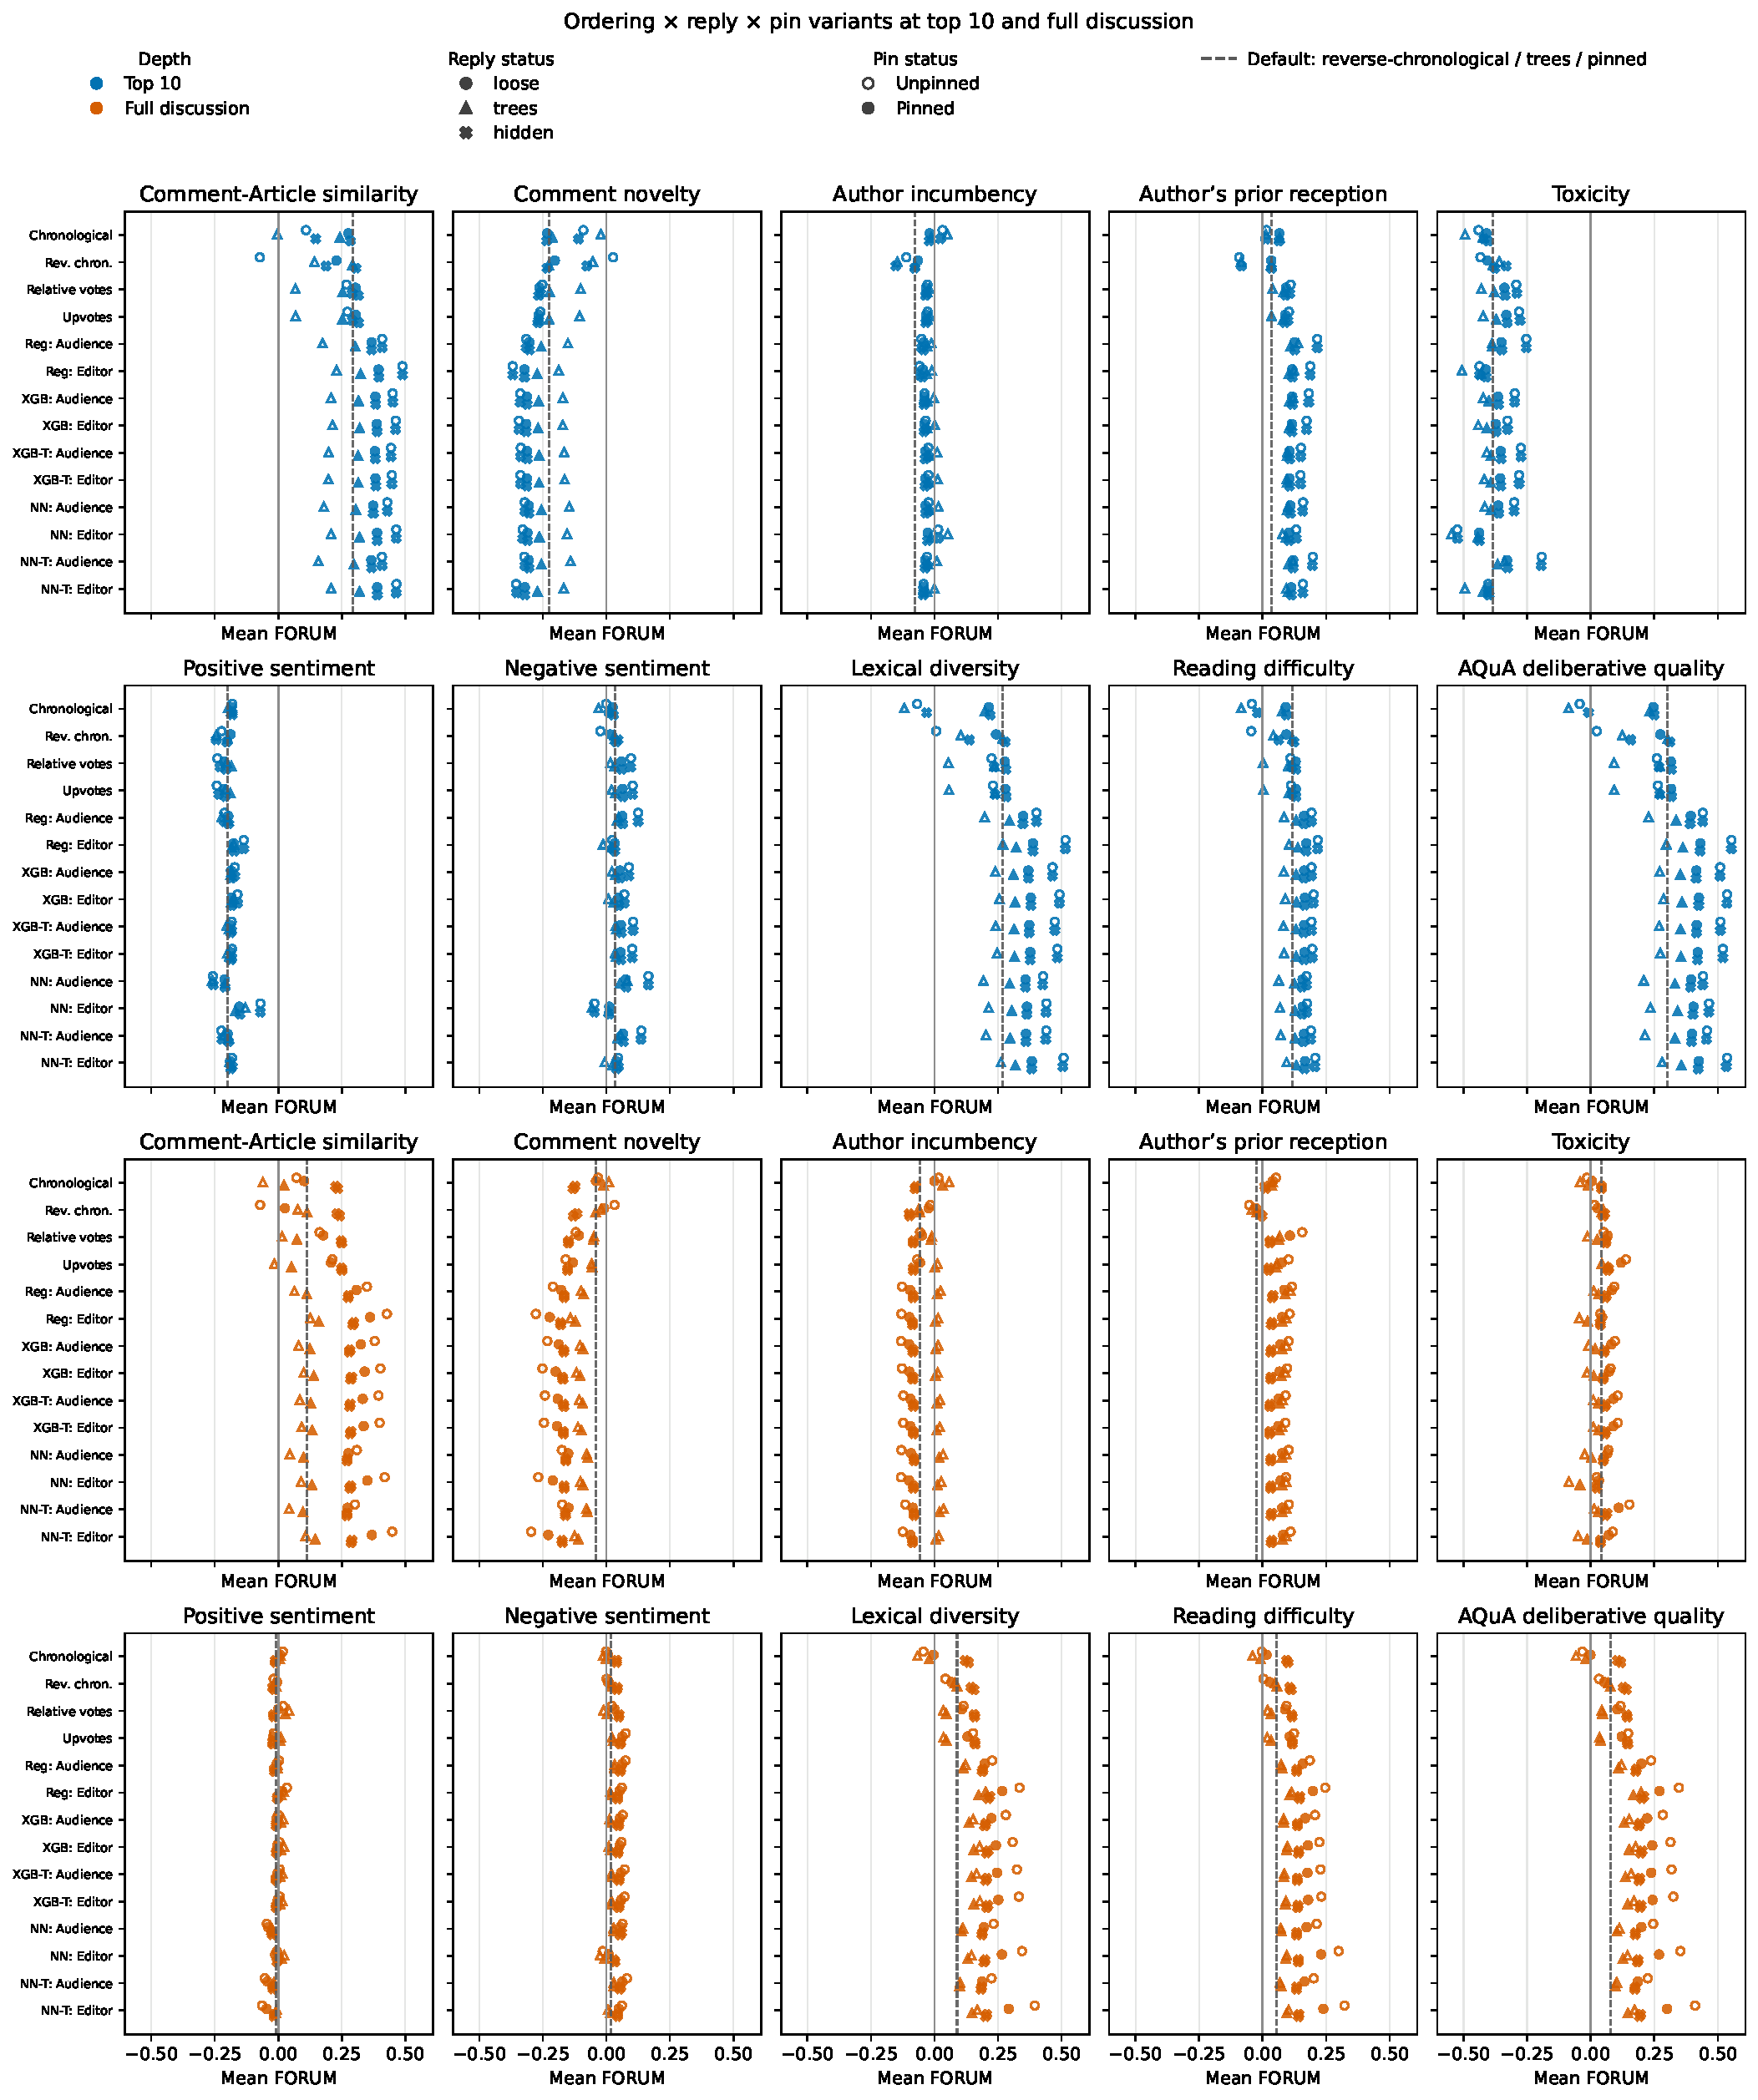
\includegraphics[width=0.90\linewidth]{figures/ordering_variants.pdf}
\caption{Detailed ordering-policy variants at top-10 and full-discussion depths, showing the six reply/pinning configurations across the ten primary feature outcomes. Positive FORUM values indicate prominence above the expected random trajectory and negative values indicate suppression. Dashed grey lines mark the complete default presentation (reverse-chronological ordering, reply trees, and pinned Editors' Picks). These are feature-specific outcomes, not a single quality ranking.}
\label{fig:ordering-variants}
\end{figure*}

\begin{figure*}[t]
\centering
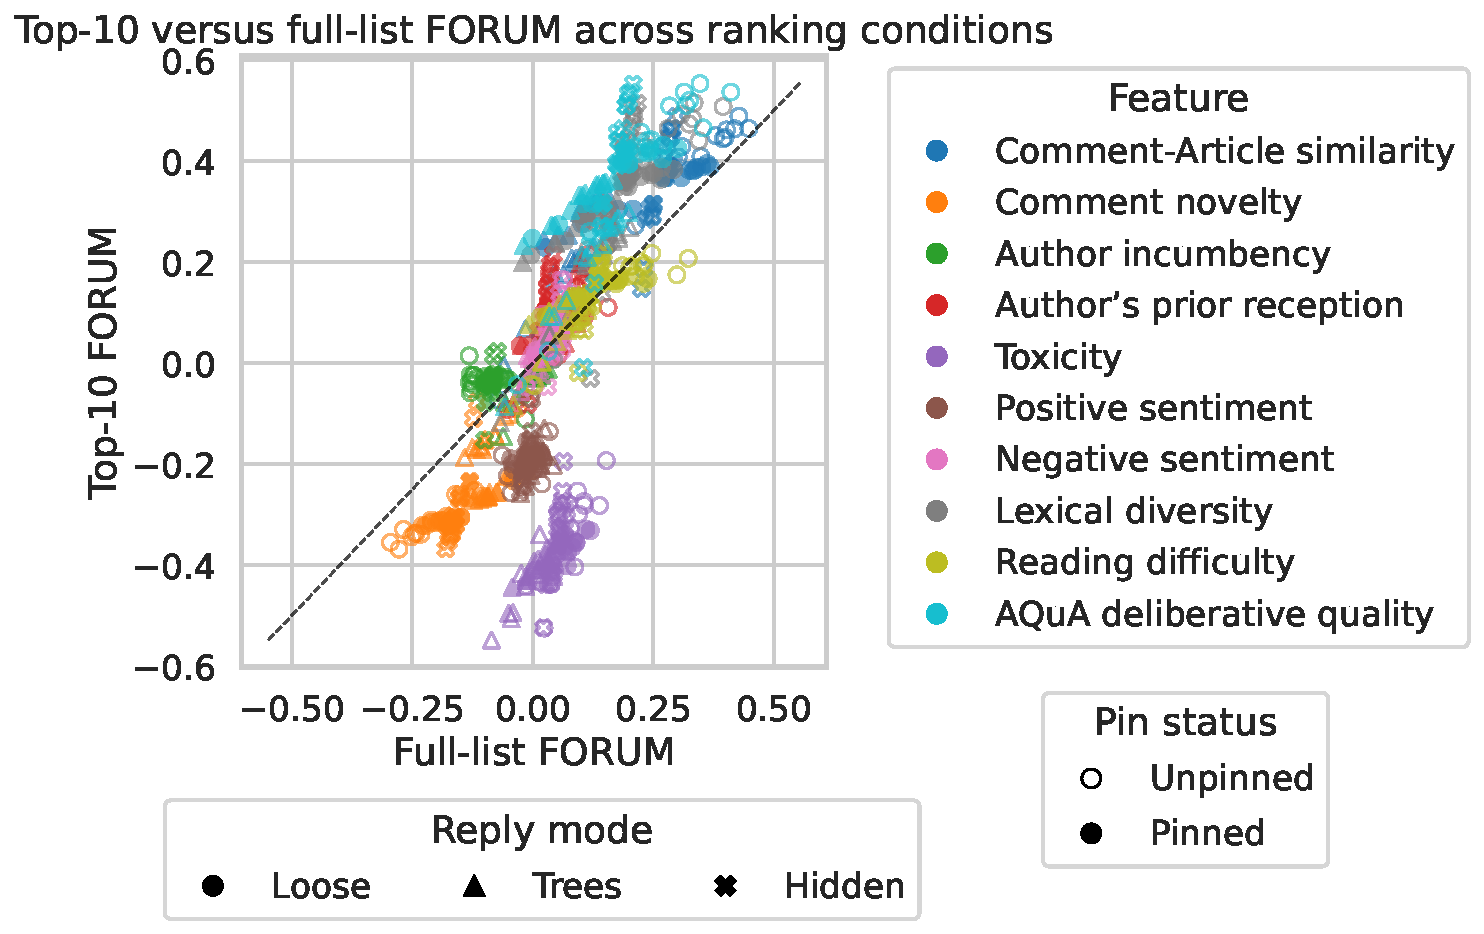
\includegraphics[width=\linewidth]{figures/forum_top10_full_across_ranking_conditions.pdf}
\caption{Top-10 versus full-discussion FORUM across ranking conditions. Each point is one of the 84 substantive policy bundles paired with one of the ten primary outcomes; the horizontal axis is full-list FORUM and the vertical axis is top-10 FORUM. Colour identifies the feature, marker shape reply mode, and fill pinning. The dashed line marks equality.}
\label{fig:forum-top10-full}
\end{figure*}


\section{Predictors and Model Development}
\label{app:development}
\label{app:feature-operationalisation}
Table~\ref{tab:model-features} details the common predictor set introduced in the ``Constructing ranking algorithms'' subsection. Numeric predictors are standardised using development data; binary indicators remain on the $0$--$1$ scale. Predictor novelty uses only earlier comments; the novelty outcome in Table~\ref{tab:outcome-features} instead uses the completed discussion.

Model development uses the article split and five cross-validation folds. Audience labels resolve relative-vote cutoff ties using the first of ten reproducible draws; editorial labels are observed Editors' Picks. Each selector has the same number of positive labels within an article.

The conditional-logit model uses article--selector strata and selector-by-feature interactions. XGBoost uses a shared LambdaRank ensemble with a selector indicator. A two-stage hyperparameter search selects models by mean article-level nDCG@$k$ across selectors and development folds, where $k$ is the number of selected comments in the article. The scalar model has 225 depth-six trees; the text-enabled model has 291 depth-five trees.

The neural models have separate audience and editor prediction heads. Scalar inputs are projected to 128 dimensions; the text-enabled variant additionally projects BGE-M3 embeddings to 256 dimensions. Each head has a 128-unit hidden layer and dropout 0.10. Training uses pairwise logistic loss with four sampled non-selected comments per selected comment and development-fold early stopping. Final fits use the median fold-selected duration: nine epochs for the scalar model and twelve for the text-enabled model. All models are frozen before held-out scoring.

\section{Detailed Ordering-Policy Effects}
\label{app:ordering}
Figure~\ref{fig:ordering-variants} shows FORUM scores for each ordering, reply, and pinning combination at both depths. These policy-specific scores complement the average contrasts in the main text, which can conceal differences between configurations.

\subsection{Comparison with nDCG}

Normalised discounted cumulative gain (nDCG) compares discounted feature values with an ideal ordering \citep{Wang2013}. For feature values $x_k$ and policy order $\pi_p$, let
\begin{equation}
\begin{aligned}
z_k&=\frac{x_k-\min_\ell x_\ell}{\max_\ell x_\ell-\min_\ell x_\ell},\\
\operatorname{nDCG}_d^p&=
\frac{\sum_{i=1}^{d}z_{\pi_p(i)}/\log_2(i+1)}
{\sum_{i=1}^{d}z_{\pi_b(i)}/\log_2(i+1)}.
\end{aligned}
\end{equation}
where $z_k$ is min--max transformed relevance for comment $k$, $d$ is the evaluation depth, $\pi_p(i)$ is the comment at rank $i$ under policy $p$, and $\pi_b$ orders comments by descending $x_k$. We use $d=10$ and $d=N-1$, matching the FORUM horizons. Discussions with constant feature values are excluded from the corresponding comparison because the relevance transformation is undefined. When a policy hides comments, nDCG preserves the visible prefix and appends omitted comments in ranked-root order, retaining the stored parent-before-child traversal within each root. This differs from FORUM's linear continuation for hidden material.

\subsection{Agreement across depths and measures}
Across the 84 substantive policy bundles and ten primary outcomes, top-10 and full-discussion FORUM correlate at $r=0.773$ and Spearman $\rho=0.811$ (Fig. \ref{fig:forum-top10-full}). Feature-specific Spearman correlations are lower for positive sentiment ($0.476$) and prior reception balance ($0.372$) than for article similarity ($0.894$) and lexical diversity ($0.877$). Early prominence is therefore not interchangeable with full-list presentation---topical similarity and lexical diversity are relatively stable across horizons, whereas positive sentiment and prior reception balance are more horizon-dependent.

Across policy--feature combinations, FORUM and nDCG correlate more strongly at top 10 ($r=0.901$, $\rho=0.895$) than at full depth ($r=0.262$, $\rho=0.538$; Fig.~\ref{fig:forum-ndcg}). Full-depth agreement remains feature-dependent: Spearman correlations are $0.644$ for positive sentiment, $0.724$ for prior reception balance, and $0.975$ for article similarity. The measures answer different questions. nDCG discounts lower ranks and measures recovery of ideal feature values; FORUM averages signed, normalised deviations from the expected random trajectory.

\begin{figure*}[t]
\centering
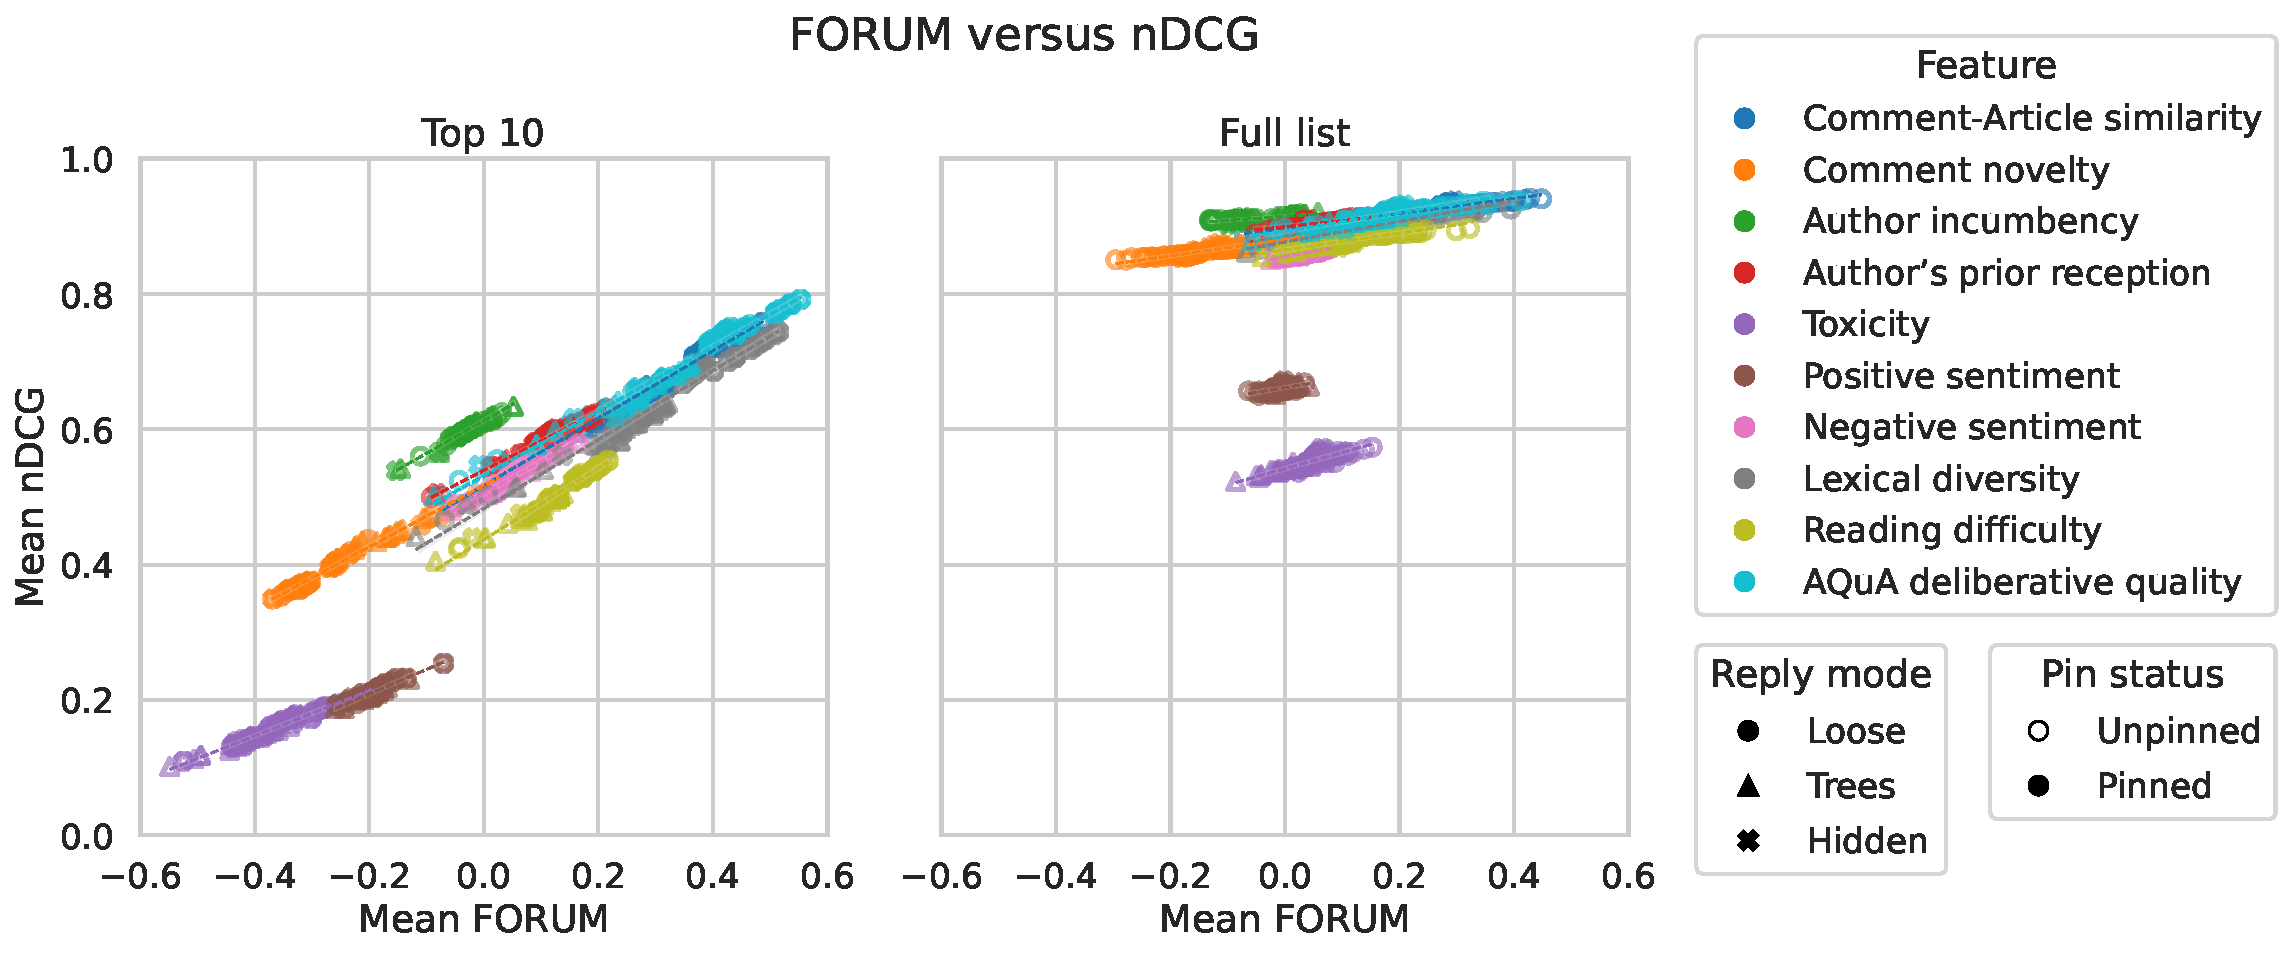
\includegraphics[width=\linewidth]{figures/forum_vs_ndcg_by_depth.pdf}
\caption{FORUM versus direct nDCG by depth. Each point is one of the 84 substantive policy bundles paired with one of the ten primary outcomes; panels separate top-10 and full-list values. FORUM is on the horizontal axis and nDCG on the vertical axis. Colour identifies the feature, marker shape reply mode, and fill pinning.}
\label{fig:forum-ndcg}
\end{figure*}

\section{Topic-Model Selection}
\label{app:topic-model}
The topic-model search uses a fixed mixed corpus of 48,887 article passages and 48,887 sampled comments. It evaluates 60 combinations of minimum cluster size, UMAP neighbourhood size, and minimum samples, with three seeds (2025--2027), for 180 fits. Figure~\ref{fig:topic-selection} reports article-passage and sampled-comment assignment coverage and the median pooled adjusted mutual information (AMI) among documents assigned in both runs of each seed pair. This stability measure is conditional and does not indicate that every document receives a stable topic.

The selected setting (minimum cluster size 15, ten neighbours, minimum samples 5, seed 2026) lies on the coverage--stability frontier: no other setting improves one of the three diagnostics without worsening another. Its median pooled common Adjusted Mutual Information (AMI) is 0.669, with raw fit-assignment coverage of 58.60\% for article passages and 33.56\% for sampled comments. The qualitative choice also considered top topic coherence and topic count, the number of documents in very small topics, and relative improvement across these diagnostics. The selected setting has a median 719 pre-reduction topics and zero pooled documents in topics of size at most 5 or 10. A neighbouring frontier setting (minimum cluster size 10, 15 neighbours, minimum samples 3) has similar coverage (59.88\% and 33.56\%) and AMI (0.666), but 1,255 topics and 1,160 pooled documents in topics of size at most 10. The final 439-topic model and its assignment coverage are reported in the ``Measuring the presented topic agenda'' subsection. Its coverage of 53.59\% for article passages and 26.64\% for candidate comments comes from applying the final model to the full article and comment corpus.
\begin{figure*}[t]
\centering
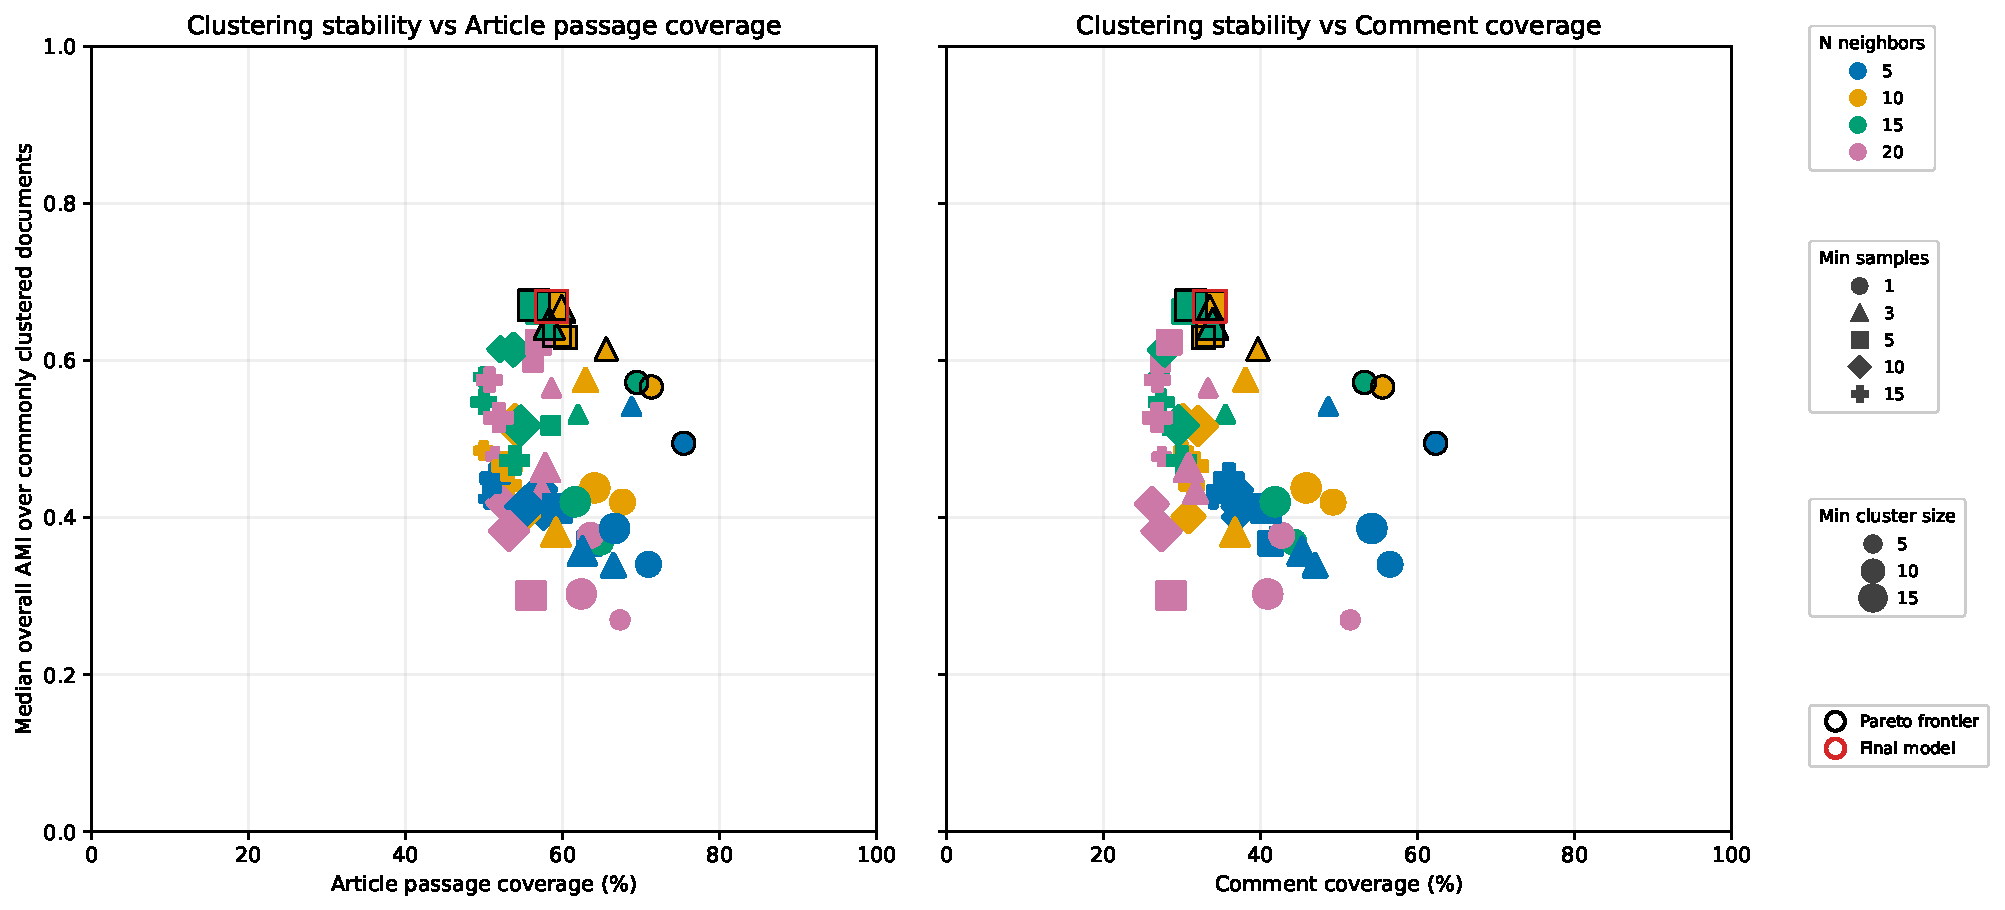
\includegraphics[width=\linewidth]{figures/topic_stability_coverage.pdf}
\caption{Topic clustering stability versus article and sampled-comment coverage. The two panels share median pooled common-assignment AMI and distinguish the two coverage denominators. Open markers identify the three-objective Pareto frontier; the red outline marks the selected setting.}
\label{fig:topic-selection}
\end{figure*}

\section{Development Vote-Activity Weights}
\label{app:attention}
The reconstructed development presentations contain 1,189,267 candidate comments across 2,553 discussions. Pinning hides 146,950 descendants, leaving 1,042,317 visible comments and 7,634,736 recorded votes. No zero-vote discussion is excluded. Within each discussion, vote fractions sum to one and absent ranks contribute zero. Conditioning the fit on visible length separates rank weighting from the declining number of discussions that reach later ranks.

The log-weight spline described in the ``Measuring the presented topic agenda'' subsection uses denser knots near the start of the list. Nested development-fold validation selects a second-difference penalty of $10^{-4}$. Mean per-story validation cross entropy is 5.411 nats for the selected spline, versus 5.507 for a fitted power law and 5.606 for a fitted exponential. The latter curves are development-fit comparators in Figure~\ref{fig:attention-fit}; presented agenda analyses use the spline only, though these alternatives give qualitatively similar results. 
\section{Asset Licences}
\label{app:licences}
The following records identify the upstream licences of the pretrained assets used for feature extraction (checked 16 September 2026).
\begin{itemize}
\item \textbf{BGE-M3:} \texttt{BAAI/bge-m3} is released under the MIT licence, as declared in its model card: \url{https://huggingface.co/BAAI/bge-m3}.
\item \textbf{Sentiment:} the official XLM-T repository associated with \path{cardiffnlp/twitter-xlm-roberta-base-sentiment} carries the Apache License 2.0: \url{https://github.com/cardiffnlp/xlm-t/blob/main/LICENSE}.
\item \textbf{AQuA:} the upstream repository containing the deliberative-quality code and trained adapters carries the Apache License 2.0: \url{https://github.com/mabehrendt/AQuA}.
\item \textbf{Toxicity:} \path{textdetox/xlmr-large-toxicity-classifier-v2} declares OpenRAIL++ (\texttt{openrail++}) in its model card: \url{https://huggingface.co/textdetox/xlmr-large-toxicity-classifier-v2}.
\end{itemize}

\section{Compute Resources}
\label{app:hardware}
The computational experiments ran on a Linux workstation with an AMD Ryzen 9
9950X processor (16 physical cores, 32 hardware threads) and 64~GB installed
system memory (approximately 60~GiB visible to the operating system). GPU
workloads used one NVIDIA RTX A5000 with 24~GB VRAM.

\begin{figure*}[t]
\centering
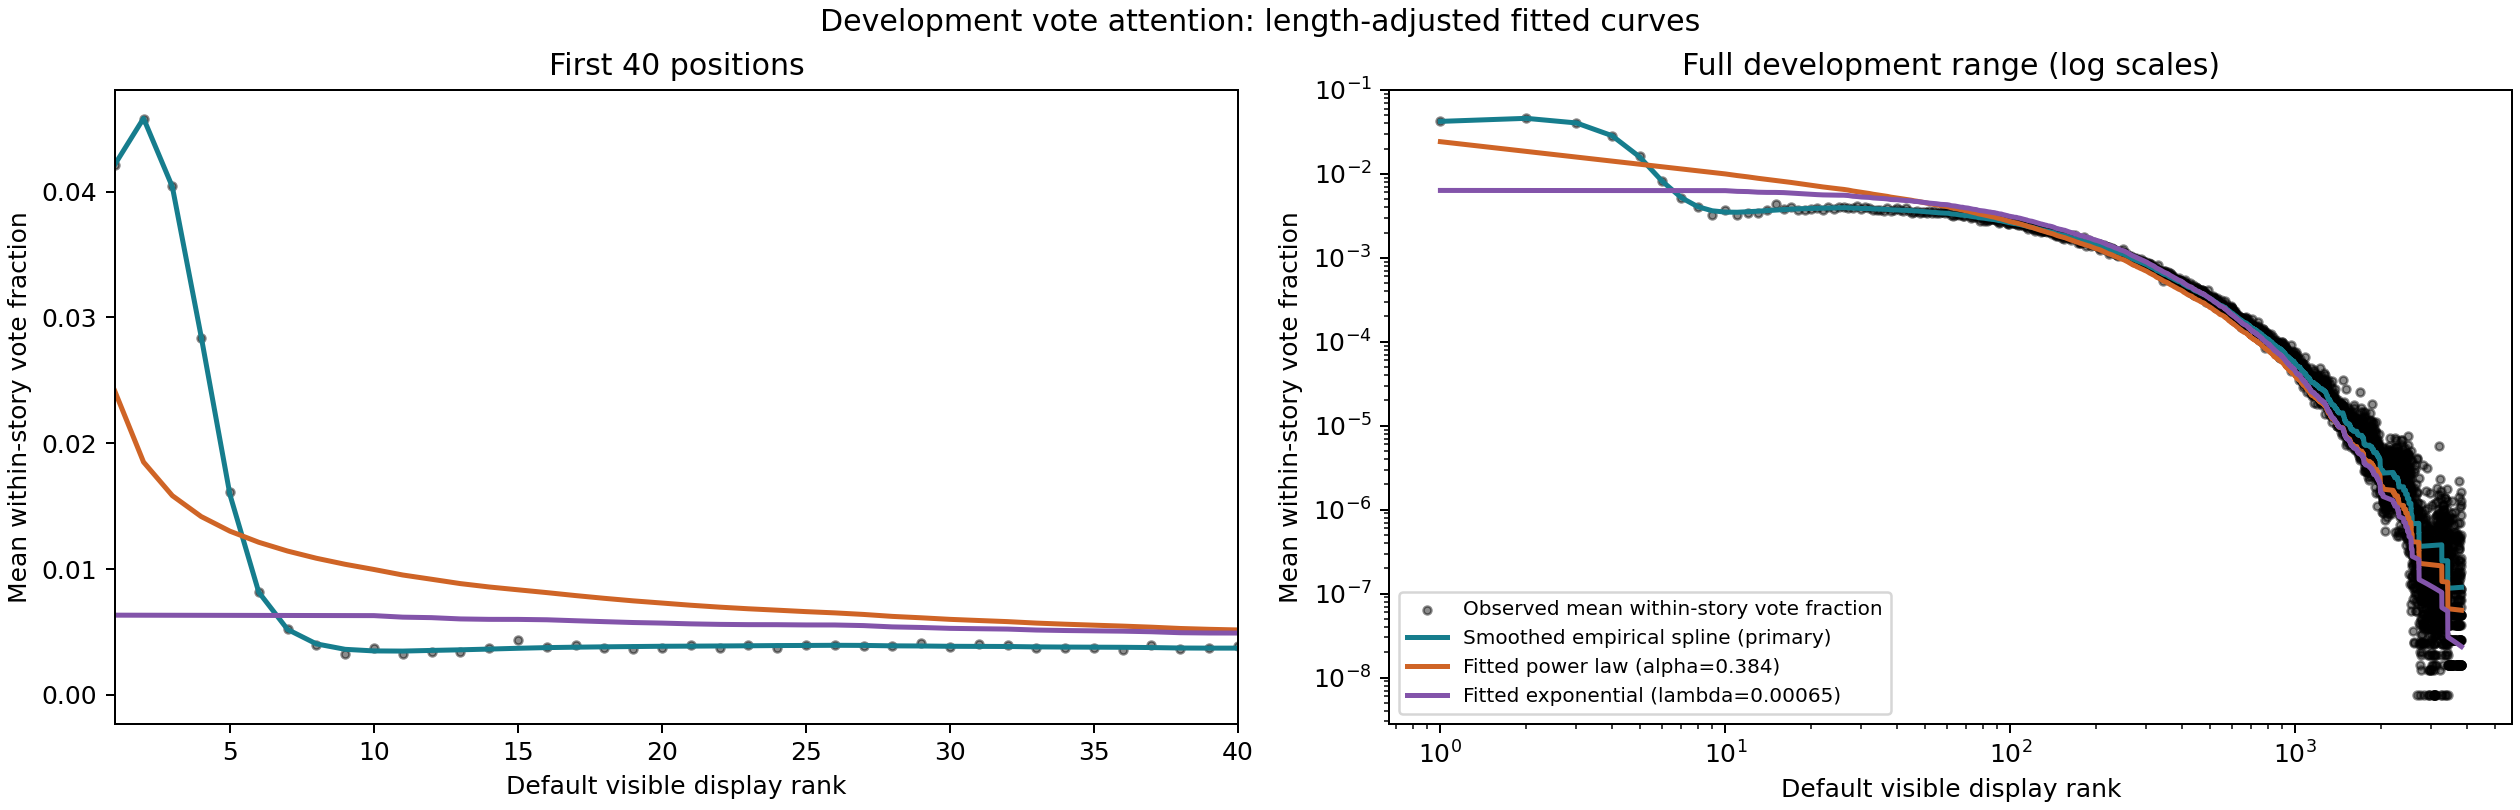
\includegraphics[width=\linewidth]{figures/development_vote_attention.png}
\caption{Development vote activity and length-adjusted fitted curves. The first forty positions are shown on linear axes and the full range on log--log axes. Empirical values are equal-discussion mean within-story vote fractions; fitted curves account for visible discussion length. The spline supplies the agenda-analysis weights.}
\label{fig:attention-fit}
\end{figure*}
